\documentclass{article}
\usepackage[utf8]{inputenc}
\usepackage{geometry}
\geometry{letterpaper, portrait, margin=1in}

\title{Traviz: Visualization of Traces in Distributed Systems}
\author{Vaastav Anand \\ vaastav.anand05@gmail.com  \and Matheus Stolet \\ stolet@cs.ubc.ca}

\date{}

\usepackage{natbib}
\usepackage{graphicx}

\begin{document}

\maketitle

\section{Introduction}

Distributed systems form the backbone of many modern applications. The Google search engine,
YouTube, Facebook, and even the mediocre web app built by your neighbor's prodigy kid touches
a distributed system in some way. These systems form much of the mission critical infrastructure
of modern computing and are comprised of multiple nodes with complex communication patterns. Because
of the importance and complexity of distributed systems, it is crucial for the developers building
them to identify performance bottlenecks and visualize different communication patterns. 

A technique used to better understand distributed systems is tracing. A trace represents the
path of one request through the system and contains information such as the timing of requests, 
the events executed, and the nodes where these events were executed. Moreover, traces can be used
to identify slow requests and understand the difference between request executions. In this project, we
propose to create a visualization tool that uses data from traces to succintly represent the structure 
and performance of a distributed system. Our tool will allow users to compare the path taken by a group
of requests to the path taken by other requests. We believe that a visualization tool that can represent the
structure of a trace, while also visually encoding information relevant for understanding performance,
will make distributed systems more understandable and debuggable.

Both of us have experience with the problem domain. Vaastav has been working on distributed systems for years
and participated in many different projects in the area. Furthermore, his recent research has investigated
tracing in distributed systems. Matheus also has experience with distributed systems through coursework,
research assistanships and graduate research. Tracing is a new topic for him, but he has found it to be
an interesting area that can be useful for debugging and comprehending the interactions of large networks
of computers.

\section{Data}

We have a collection of traces and source code for a couple of different systems. Our traces come from two datasets.
The first dataset is called HDFS and contains the traces from a file system in Hadoop used for distributed storage 
and big data processing. This dataset has a total of 71,001 traces. The second dataset is called socialNetwork and
was obtained from the DeathStarBench open-source benchmark for cloud microservices. The traces of this dataset model
the microservices of a social network composed of multiple individual applications. The socialNetwork dataset has
a total of 22,286 traces. The attributes of both datasets model five different entities: traces, events, hosts,
processes and threads. These entities are illustrated in \ref{fig:entities}.

\begin{figure}
    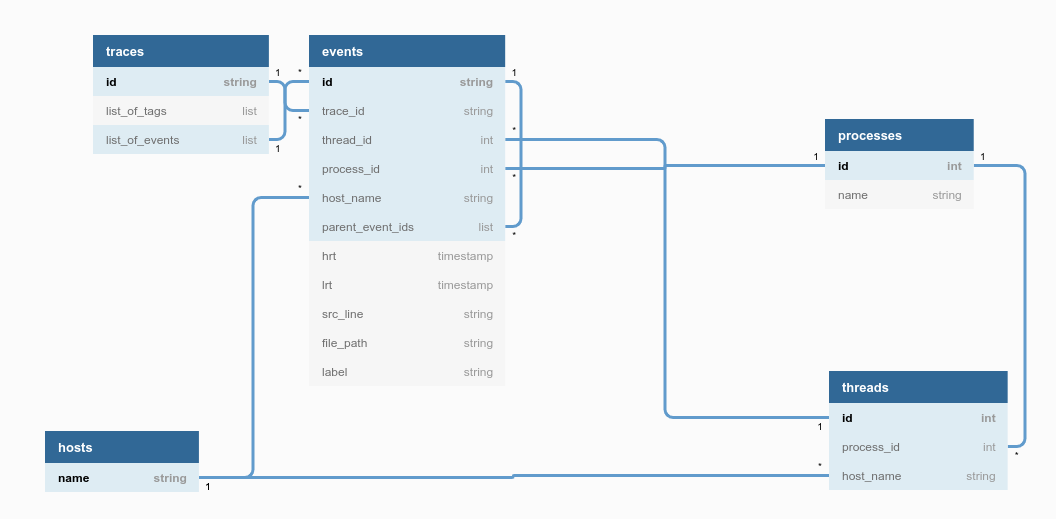
\includegraphics[width=\linewidth]{../data_abstractions.png}
    \caption{The different entities in TraViz.}
    \label{fig:entities}
  \end{figure}

\subsection{Trace}

A trace is a collection of events. It represents a request from a client to a service and shows the path of the
request through the microservice. A trace has three attributes: \textit{id}, \textit{list\_of\_tags}, and \textit{list\_of\_events}.
The \textit{id} of the trace is used to identify a trace. The \textit{list\_of\_tags} is a list of human defined keywords that serve as
the metadata for the trace. There are on average two tags per trace in both datasets, but the socialNetwork
dataset has a total of 8 different tags and the HDFS dataset has a total of 22285 different tags. The
\textit{list\_of\_events} attribute is a list of the events that happened in a trace. The events in the list
are ordered, with events that caused another event preceding the caused event in the list. The causal relationship
between the events forms a DAG. There are around 100 events per trace in the socialNetwork dataset and 1400 events per trace
in the HDFS dataset.

\subsection{Event}

\subsection{Host}

A host represents a node in the distributed system. It encapsulates the processes and threads
that execute the events in a trace. There are 13 different hosts across the social network dataset
and 9 different hosts across the HDFS dataset. The host is identified by a name attribute, which is
referenced by events and threads.

\subsection{Process}

The process entity represents a operating system process running on
a host. Processes have an \textit{id} attribute, which is referenced by the events and threads executed in
the process. The process also has a \textit{name} attribute, which gives a human understandable name for the
application running the process. There are around 20 different processes per trace in the socialNetwork
dataset and 18 different processes per trace in the HDFS dataset. There are 13 different process names
in the socialNetwork dataset and 4 different process names in the HDFS dataset.

\subsection{Thread}

The thread entity represents
a kernel or user thread. Distinguishing between both is not important for the purposes of this project, so we
simply see it as the basic unit of execution. Threads have an \textit{id} attribute that identifies a thread
within a trace. Events use the \textit{id} to signal the thread that executed them. It is important to note
that the thread \textit{id} does not match across traces, and the total number of threads is not useful because it's
not possible to correlate them between traces. Each thread also has a \textit{host\_name} and \textit{process\_id}
attribute. These attributes are used to identify the host and process that executed a thread. 

\section{Task}

\section{Proposed Solution}

\section{Implementation Approach}

\section{Schedule}

\section{Related Work}

\end{document}

